\documentclass[border=5pt]{standalone}
\usepackage{tikz}
\usetikzlibrary{arrows.meta,positioning}
\definecolor{blue}{HTML}{0072B2}
\definecolor{orange}{HTML}{D55E00}
\tikzset{
  >={Stealth[length=5pt]},
  box/.style={draw=black!70,rounded corners=2pt,align=center,minimum height=14mm,text width=27mm,inner sep=5pt,font=\sffamily\small},
  flow/.style={->,line width=.8pt,draw=black!75},
  note/.style={font=\sffamily\scriptsize,align=center,text=black!75}
}
\begin{document}
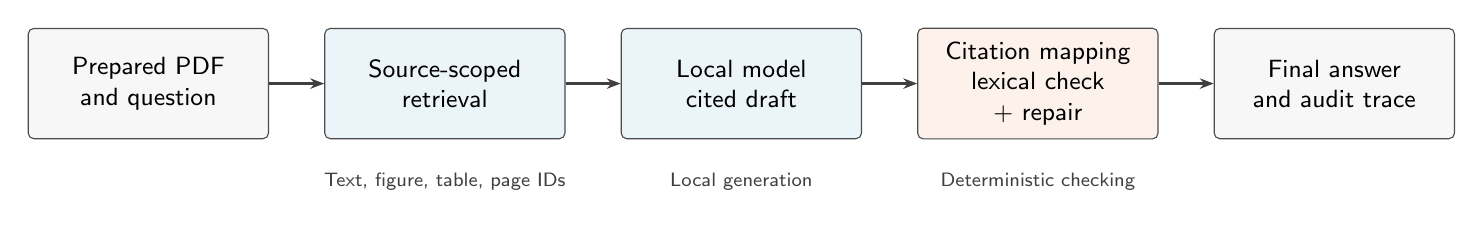
\begin{tikzpicture}[node distance=7mm]
  \node[box,fill=black!3] (input) {Prepared PDF\\and question};
  \node[box,fill=blue!8,right=of input] (retrieve) {Source-scoped\\retrieval};
  \node[box,fill=blue!8,right=of retrieve] (generate) {Local model\\cited draft};
  \node[box,fill=orange!8,right=of generate] (repair) {Citation mapping\\lexical check + repair};
  \node[box,fill=black!3,right=of repair] (output) {Final answer\\and audit trace};
  \draw[flow] (input) -- (retrieve);
  \draw[flow] (retrieve) -- (generate);
  \draw[flow] (generate) -- (repair);
  \draw[flow] (repair) -- (output);
  \node[note,below=3mm of retrieve] {Text, figure, table, page IDs};
  \node[note,below=3mm of generate] {Local generation};
  \node[note,below=3mm of repair] {Deterministic checking};
\end{tikzpicture}
\end{document}
